%
% teil1.tex -- Beispiel-File für das Paper
%
% (c) 2020 Prof Dr Andreas Müller, Hochschule Rapperswil
%
\section{Problemstellung}
\rhead{Problemstellung}
Wegen der breiten Anwendung der Matrizenmultiplikation ist eine effiziente L\"osung dieser Operation von grosser Bedeutung.
Das Ziel dieses Papers ist, verschiedenen Algorithmen der Matrizenmultiplikation vorzustellen.
Gezielt wird auf Algorithmen eingegangen, welche das Problem schneller als der Standard Algorithmus l\"osen.

\subsection{Big $\mathcal{O}$ Notation}
\label{muliplikation:sec:bigo}
Die Big $\mathcal{O}$ Notation beschreibt die Laufzeitkomplexit\"at eines Algorithmus in Abhängigkeit zur Inputgrösse \cite{multiplikation:bigo}.
$f(x) \in \mathcal{O}(g(x))$ besagt, dass die Funktion $f$ nicht wesentlich schneller w\"achst als $g$ wenn $x \rightarrow \infty$.
% Es gibt eine Konstante $K$ derart, dass $f(x) \le K g(x)$ für $x\to\infty$
Als Beispiel: benötigt eine Funktion $g$ $\mathcal{O} (n^2  )$ Multiplikationen, so wächst $f$ mit $\mathcal{O} (n+ n^2  )$ nicht wesentlich schneller falls $x\to\infty$.
Vereinfacht werden f\"ur Algorithmen die folgende Notation verwendet:
\begin{itemize}
	\item $f \in \mathcal{O}(1) \rightarrow f$ ist beschr\"ankt
	\item $f \in \mathcal{O}(n) \rightarrow f$ w\"achst linear
	\item $f \in \mathcal{O}  (n^2   ) \rightarrow f$ w\"achst quadratisch
	\item $f \in \mathcal{O}(\log n) \rightarrow f$ w\"achst logarithmisch
	\item $f \in \mathcal{O}(n \log n) \rightarrow f$ hat super-lineares Wachstum
	\item $f \in \mathcal{O}  (e^n   ) \rightarrow f$ w\"achst exponentiell
	\item usw.
\end{itemize}

In der Abbildung \ref{multiplikation:fig:bigo} k\"onnen die verschiedenen Laufzeiten miteinander verglichen werden.
Bei einer logarithmischen Darstellung werden Polynome der Form $f(x) = x^k$ als Gerade und Exponentialfunktionen der Form $f(x) = a^x$ als nach oben gekr\"ummte Kurven dargestellt.



\subsubsection{Beispiel Algorithmen}

Es folgen einige Beispiele von Algorithmen welche zu einer bestimmten Zeitkomplexit\"atsklasse zugeteilt werden k\"onnen.


\begin{table}[t]
	\begin{tabular}{ll}
		\begin{minipage}{0.48\textwidth}
			\begin{algorithm}[H]\footnotesize\caption{}
				\label{multiplikation:alg:b1}
				\setlength{\lineskip}{7pt}
				\begin{algorithmic}
					\Function{B1}{$a, b$}
					\State \textbf{return} $a+b$
					\EndFunction
					\State
					\State
				\end{algorithmic}
			\end{algorithm}
		\end{minipage}	
		&
		\begin{minipage}{0.48\textwidth}
			\begin{algorithm}[H]\footnotesize\caption{}
				\label{multiplikation:alg:b2}
				\setlength{\lineskip}{7pt}
				\begin{algorithmic}
					\Function{B2}{$a, b$}
					\State $ x \gets a+b $
					\State $ y \gets a \cdot b $
					\State \textbf{return} $x+y$
					\EndFunction
				\end{algorithmic}
			\end{algorithm}
			
		\end{minipage}
	\end{tabular}
\end{table}

\begin{table}
	\begin{tabular}[t]{ll} 
		\begin{minipage}{0.48\textwidth}
			\begin{algorithm}[H]\footnotesize\caption{}
				\setlength{\lineskip}{7pt}
				\begin{algorithmic}
					\label{multiplikation:alg:linear}
					\Function{L}{$\mathbf{a}, \mathbf{b}$,n}
					\State $ sum \gets 0$
					\For{$i = 0,1,2 \dots,n$}
					\State $ sum \gets sum + A[i] \cdot B[i] $
					\EndFor
					
					\State \textbf{return} $sum$
					
					\EndFunction
					\State
					\State
				\end{algorithmic}
			\end{algorithm}
		\end{minipage}	
		&
		\begin{minipage}{0.48\textwidth}
			\begin{algorithm}[H]\footnotesize\caption{}
				\label{multiplikation:alg:q1}
				\setlength{\lineskip}{7pt}
				\begin{algorithmic}
					\Function{Q}{$\mathbf{A}, \mathbf{B}$,n}
					\State $ sum \gets 0$
					\For{$i = 0,1,2 \dots,n$}
					\For{$j = 0,1,2 \dots,n$}
					\State $ sum \gets sum + A[i] \cdot B[j] $
					\EndFor
					\EndFor
					\State \textbf{return} $sum$
					\EndFunction
				\end{algorithmic}
			\end{algorithm}
		\end{minipage}
	\end{tabular}
\end{table}

\paragraph{Beschr\"ankter Algorithmus}

Ein Beispiel eines Beschr\"ankter Verhalten $\mathcal{O}(1)$, kann im Algorithmus \ref{multiplikation:alg:b1} entnommen werden. Da $a$ und $b$ Skalare sind, hat keine Gr\"osse $n$ einen Einfluss auf die Laufzeit.

Konstanten werden nicht beachtet, der Algorithmus \ref{multiplikation:alg:b2} f\"uhrt ebenso zu  $\mathcal{O}(1)$ und nicht zu $\mathcal{O}(2)$.


\paragraph{Linearer Algorithmus}

Der Algorithmus \ref{multiplikation:alg:linear} hat ein lineares Verhalten.
Die \texttt{for}-Schleife wird $n$-mal durchlaufen und f\"uhrt deshalb zu $\mathcal{O}(n)$.

\paragraph{Quadratischer Algorithmus}

Der Algorithmus \ref{multiplikation:alg:q1} hat ein quadratisches Verhalten.
Die beiden \texttt{for}-Schleifen werden jeweils $n$-mal durchlaufen und f\"uhrt deshalb zu $\mathcal{O} (n^2 )$.


\begin{figure}
	\center
	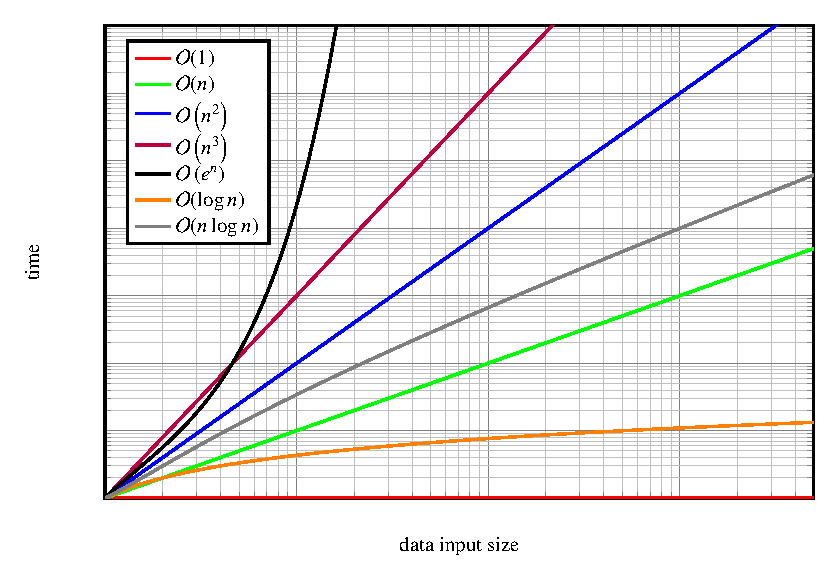
\includegraphics[]{papers/multiplikation/images/bigo}
	\caption{Verschiedene Laufzeiten}
	\label{multiplikation:fig:bigo}
\end{figure}
